
\section{Corpus Summary}
\label{cp4:corpus-summary}

This chapter main contributions are \textit{(i)} the procedures for the corpus creation, and; \textit{(ii)} the \acs{DS-android} corpus itself. A well-structured corpus lays the foundation for several studies that explore relationships between software tasks, natural language artifacts, and text within these artifacts. 

Our corpus comprises 300 tasks evenly selected from SO and Git. 
There is a total of \red{x} sentences in \red{y} artifacts pertaining API documentation, Stack Overflow answers, Github issue discussions, and miscellaneous Web tutorials or blog posts. 

--- Description of the number of task-relevant sentences in the corpus based on Section~\ref{cp4:corpus-relevant-text-ratio}



% \section{Corpus Creation}
% \label{cp4:corpus-creation}

% Corpus creation consists of three main steps, namely \textit{(1)} selection of tasks, \textit{(2)} selection of artifacts, and \textit{(3)} identification of relevant text within the selected artifacts. We detail each of these steps in the following sections.


% \subsection{Corpus Summary}
% \textcolor{white}{force ident} % this is just for the chapter outline


% Figure~\ref{fig:corpus-creation-pipeline} summarizes procedures for corpus creation.
% We randomly sample a set of Android development tasks from Stack Overflow and GitHub
% and use the Google search engine to find potential resources that might have
% information for a task. We only consider resources highly ranked at Amazon Alexa and, for these resources, we apply state of the art techniques to detect relevant text in the artifact's content.



% Our corpus comprises 300 tasks evenly selected from SO and Git. 
% There is a total of 262,278 sentences in 2,586 artifacts pertaining API documentation, Stack Overflow answers, Github issue discussions, and miscellaneous Web tutorials or blog posts. 



% \begin{figure}
%     \centering
%     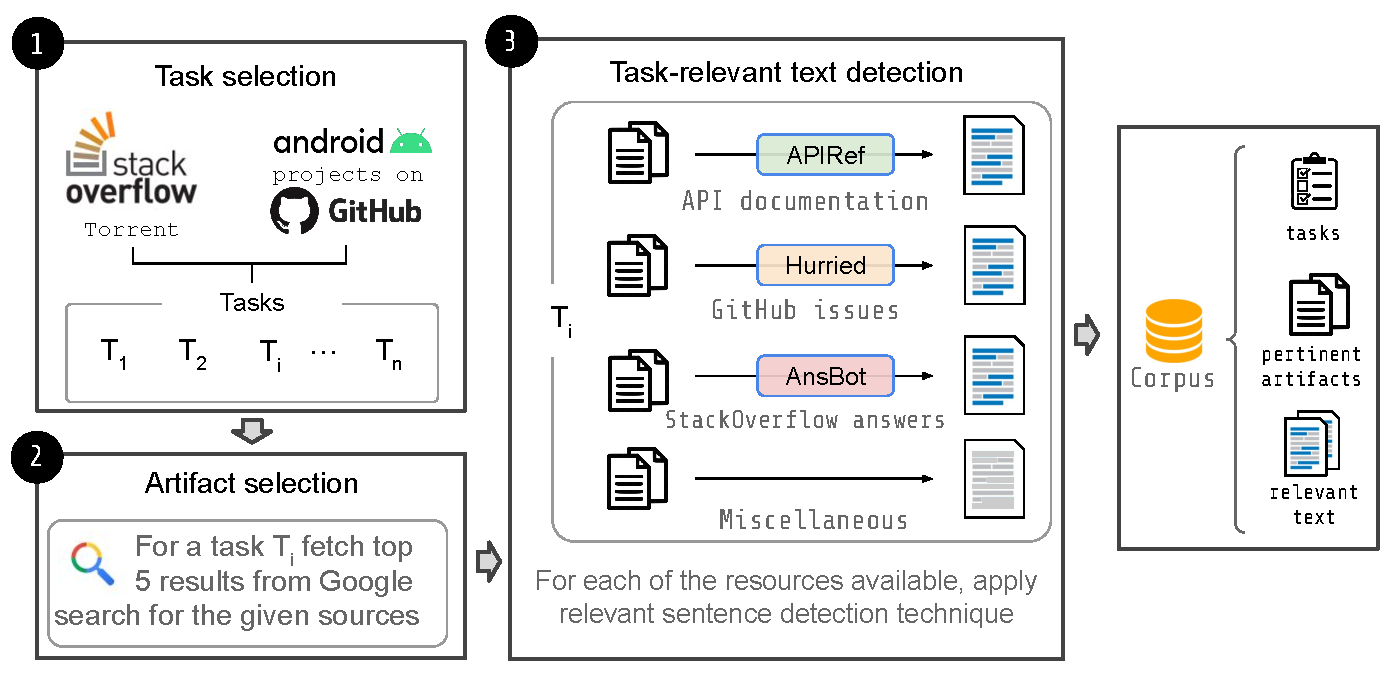
\includegraphics[width=\textwidth]{cp4/corpus-creation-pipeline}
%     \caption{Summary of procedures for corpus creation}
%     \label{fig:corpus-creation-pipeline}
% \end{figure}

